\pgfdeclareplotmark{cross} {
\pgfpathmoveto{\pgfpoint{-0.3\pgfplotmarksize}{\pgfplotmarksize}}
\pgfpathlineto{\pgfpoint{+0.3\pgfplotmarksize}{\pgfplotmarksize}}
\pgfpathlineto{\pgfpoint{+0.3\pgfplotmarksize}{0.3\pgfplotmarksize}}
\pgfpathlineto{\pgfpoint{+1\pgfplotmarksize}{0.3\pgfplotmarksize}}
\pgfpathlineto{\pgfpoint{+1\pgfplotmarksize}{-0.3\pgfplotmarksize}}
\pgfpathlineto{\pgfpoint{+0.3\pgfplotmarksize}{-0.3\pgfplotmarksize}}
\pgfpathlineto{\pgfpoint{+0.3\pgfplotmarksize}{-1.\pgfplotmarksize}}
\pgfpathlineto{\pgfpoint{-0.3\pgfplotmarksize}{-1.\pgfplotmarksize}}
\pgfpathlineto{\pgfpoint{-0.3\pgfplotmarksize}{-0.3\pgfplotmarksize}}
\pgfpathlineto{\pgfpoint{-1.\pgfplotmarksize}{-0.3\pgfplotmarksize}}
\pgfpathlineto{\pgfpoint{-1.\pgfplotmarksize}{0.3\pgfplotmarksize}}
\pgfpathlineto{\pgfpoint{-0.3\pgfplotmarksize}{0.3\pgfplotmarksize}}
\pgfpathclose
\pgfusepathqstroke
}
\pgfdeclareplotmark{cross*} {
\pgfpathmoveto{\pgfpoint{-0.3\pgfplotmarksize}{\pgfplotmarksize}}
\pgfpathlineto{\pgfpoint{+0.3\pgfplotmarksize}{\pgfplotmarksize}}
\pgfpathlineto{\pgfpoint{+0.3\pgfplotmarksize}{0.3\pgfplotmarksize}}
\pgfpathlineto{\pgfpoint{+1\pgfplotmarksize}{0.3\pgfplotmarksize}}
\pgfpathlineto{\pgfpoint{+1\pgfplotmarksize}{-0.3\pgfplotmarksize}}
\pgfpathlineto{\pgfpoint{+0.3\pgfplotmarksize}{-0.3\pgfplotmarksize}}
\pgfpathlineto{\pgfpoint{+0.3\pgfplotmarksize}{-1.\pgfplotmarksize}}
\pgfpathlineto{\pgfpoint{-0.3\pgfplotmarksize}{-1.\pgfplotmarksize}}
\pgfpathlineto{\pgfpoint{-0.3\pgfplotmarksize}{-0.3\pgfplotmarksize}}
\pgfpathlineto{\pgfpoint{-1.\pgfplotmarksize}{-0.3\pgfplotmarksize}}
\pgfpathlineto{\pgfpoint{-1.\pgfplotmarksize}{0.3\pgfplotmarksize}}
\pgfpathlineto{\pgfpoint{-0.3\pgfplotmarksize}{0.3\pgfplotmarksize}}
\pgfpathclose
\pgfusepathqfillstroke
}
\pgfdeclareplotmark{newstar} {
\pgfpathmoveto{\pgfqpoint{0pt}{\pgfplotmarksize}}
\pgfpathlineto{\pgfqpointpolar{44}{0.5\pgfplotmarksize}}
\pgfpathlineto{\pgfqpointpolar{18}{\pgfplotmarksize}}
\pgfpathlineto{\pgfqpointpolar{-20}{0.5\pgfplotmarksize}}
\pgfpathlineto{\pgfqpointpolar{-54}{\pgfplotmarksize}}
\pgfpathlineto{\pgfqpointpolar{-90}{0.5\pgfplotmarksize}}
\pgfpathlineto{\pgfqpointpolar{234}{\pgfplotmarksize}}
\pgfpathlineto{\pgfqpointpolar{198}{0.5\pgfplotmarksize}}
\pgfpathlineto{\pgfqpointpolar{162}{\pgfplotmarksize}}
\pgfpathlineto{\pgfqpointpolar{134}{0.5\pgfplotmarksize}}
\pgfpathclose
\pgfusepathqstroke
}
\pgfdeclareplotmark{newstar*} {
\pgfpathmoveto{\pgfqpoint{0pt}{\pgfplotmarksize}}
\pgfpathlineto{\pgfqpointpolar{44}{0.5\pgfplotmarksize}}
\pgfpathlineto{\pgfqpointpolar{18}{\pgfplotmarksize}}
\pgfpathlineto{\pgfqpointpolar{-20}{0.5\pgfplotmarksize}}
\pgfpathlineto{\pgfqpointpolar{-54}{\pgfplotmarksize}}
\pgfpathlineto{\pgfqpointpolar{-90}{0.5\pgfplotmarksize}}
\pgfpathlineto{\pgfqpointpolar{234}{\pgfplotmarksize}}
\pgfpathlineto{\pgfqpointpolar{198}{0.5\pgfplotmarksize}}
\pgfpathlineto{\pgfqpointpolar{162}{\pgfplotmarksize}}
\pgfpathlineto{\pgfqpointpolar{134}{0.5\pgfplotmarksize}}
\pgfpathclose
\pgfusepathqfillstroke
}
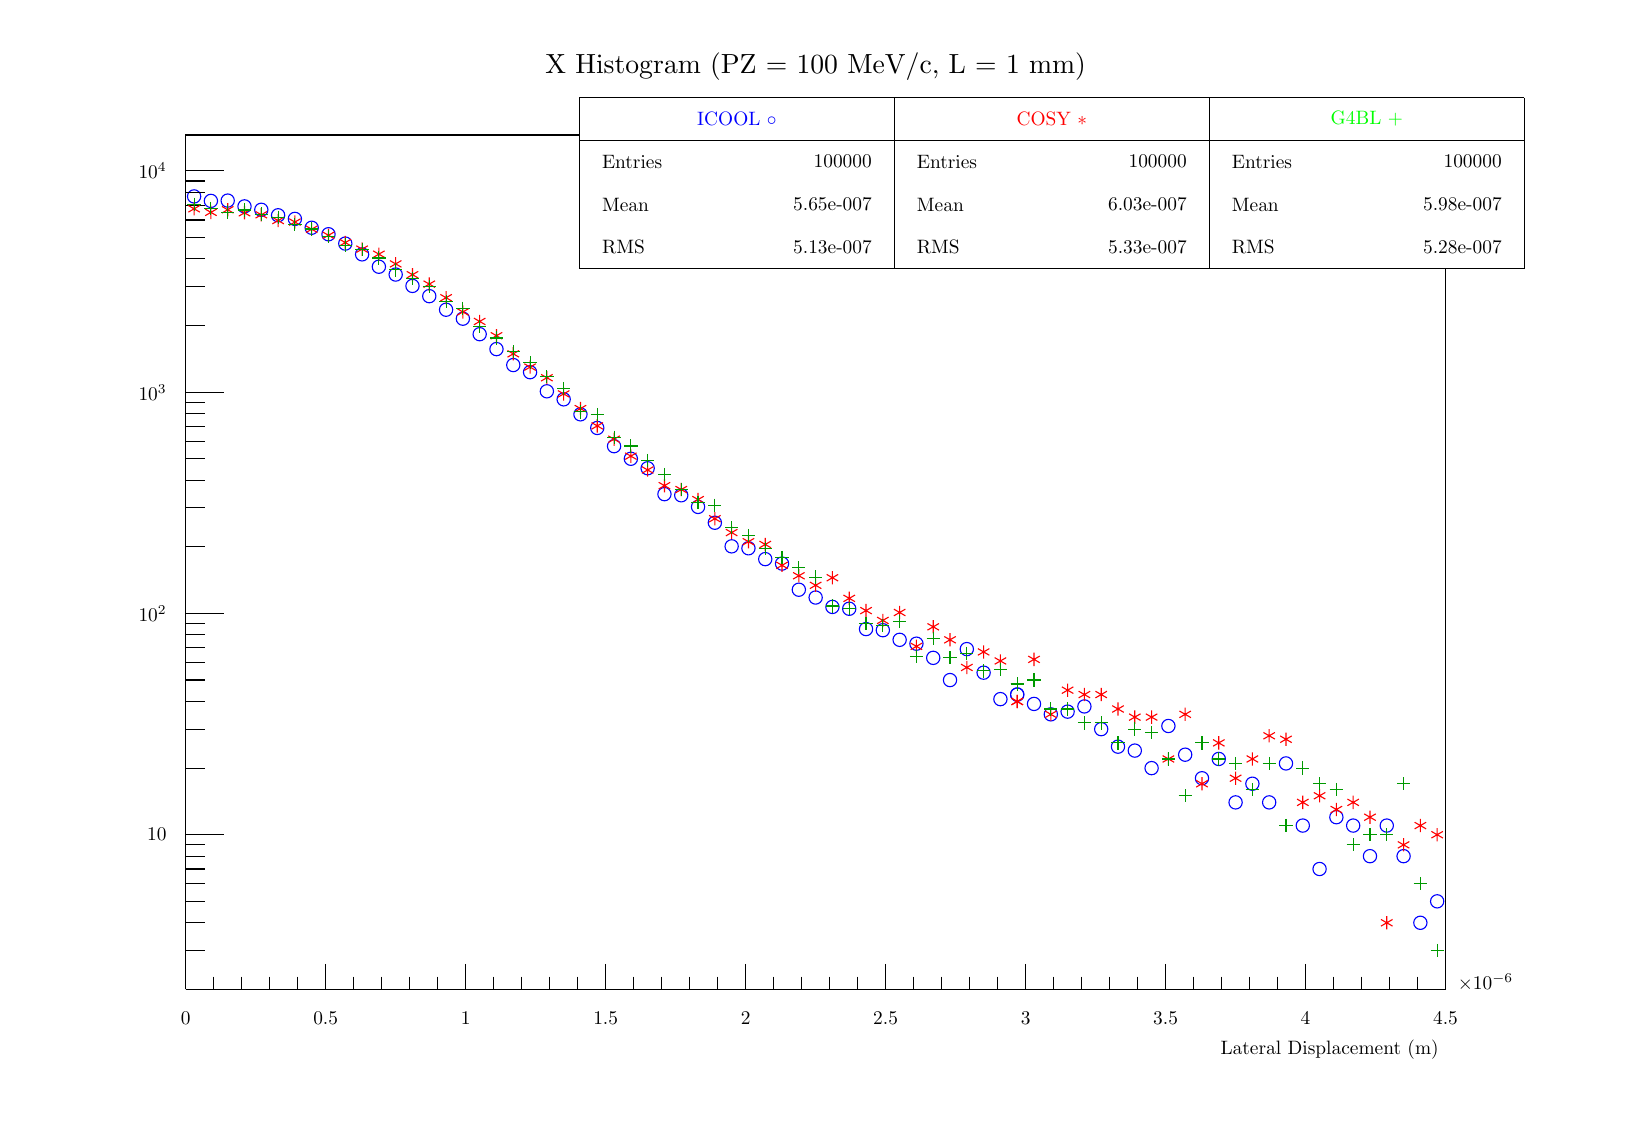
\begin{tikzpicture}
\definecolor{c}{rgb}{1,1,1};
\draw [color=c, fill=c] (0,0) rectangle (20,13.5632);
\draw [color=c, fill=c] (2,1.35632) rectangle (18,12.2069);
\definecolor{c}{rgb}{0,0,0};
\draw [c] (2,1.35632) -- (2,12.2069) -- (18,12.2069) -- (18,1.35632) -- (2,1.35632);
\definecolor{c}{rgb}{1,1,1};
\draw [color=c, fill=c] (2,1.35632) rectangle (18,12.2069);
\definecolor{c}{rgb}{0,0,0};
\draw [c] (2,1.35632) -- (2,12.2069) -- (18,12.2069) -- (18,1.35632) -- (2,1.35632);
\definecolor{c}{rgb}{0,0,1};
\foreach \P in
 {(2.10667,11.4269),(2.32,11.37),(2.53333,11.374),(2.74667,11.3003),(2.96,11.2572),(3.17333,11.1876),(3.38667,11.1414),(3.6,11.0291),(3.81333,10.9465),(4.02667,10.8281),(4.24,10.6912),(4.45333,10.534),(4.66667,10.4348),(4.88,10.2905),(5.09333,10.1602
),(5.30667,9.98813),(5.52,9.87429),(5.73333,9.67741),(5.94667,9.48782),(6.16,9.28556),(6.37333,9.19483),(6.58667,8.95212),(6.8,8.84998),(7.01333,8.65965),(7.22667,8.48653),(7.44,8.25512),(7.65333,8.0952),(7.86667,7.97472),(8.08,7.64586),(8.29333,7.63
166),(8.50667,7.48389),(8.72,7.28293),(8.93333,6.98297),(9.14667,6.95843),(9.36,6.82086),(9.57333,6.76408),(9.78667,6.43219),(10,6.33291),(10.2133,6.21348),(10.4267,6.19045),(10.64,5.93255),(10.8533,5.91811),(11.0667,5.79595),(11.28,5.7468),(11.4933,
5.56699),(11.7067,5.28492),(11.92,5.67802),(12.1333,5.37885),(12.3467,5.04272),(12.56,5.10085)}{\draw[mark options={color=c,fill=c},mark size=2.402402pt,mark=o] plot coordinates {\P};}
\foreach \P in
 {(12.56,5.10085),(12.7733,4.98168),(12.9867,4.84961),(13.2,4.88399),(13.4133,4.94998),(13.6267,4.66147),(13.84,4.43894),(14.0533,4.38912),(14.2667,4.1666),(14.48,4.70149),(14.6933,4.33718),(14.9067,4.03801),(15.12,4.28293),(15.3333,3.73128),(15.5467
,3.96825),(15.76,3.73128),(15.9733,4.22615),(16.1867,3.43695),(16.4,2.8853),(16.6133,3.54314),(16.8267,3.43695),(17.04,3.04828),(17.2533,3.43695),(17.4667,3.04828),(17.68,2.2023),(17.8933,2.47464)}{\draw[mark options={color=c,fill=c},mark
 size=2.402402pt,mark=o] plot coordinates {\P};}
\definecolor{c}{rgb}{1,1,1};
\draw [color=c, fill=c] (7,10.5115) rectangle (11,12.6816);
\definecolor{c}{rgb}{0,0,0};
\draw [c] (7,10.5115) -- (11,10.5115);
\draw [c] (11,10.5115) -- (11,12.6816);
\draw [c] (11,12.6816) -- (7,12.6816);
\draw [c] (7,12.6816) -- (7,10.5115);
\draw[color=blue](9,12.4103) node[scale=0.7, rotate=0]{ICOOL $\circ$};
\draw [c] (7,12.1391) -- (11,12.1391);
\draw [anchor= west] (7.2,11.8678) node[scale=0.6, rotate=0]{Entries };
\draw [anchor= east] (10.8,11.8678) node[scale=0.6, rotate=0]{ 100000};
\draw [anchor= west] (7.2,11.3253) node[scale=0.6, rotate=0]{Mean  };
\draw [anchor= east] (10.8,11.3253) node[scale=0.6, rotate=0]{ 5.65e-007};
\draw [anchor= west] (7.2,10.7828) node[scale=0.6, rotate=0]{RMS   };
\draw [anchor= east] (10.8,10.7828) node[scale=0.6, rotate=0]{ 5.13e-007};
\draw [c] (2,1.35632) -- (18,1.35632);
\draw [anchor= east] (18,0.596782) node[scale=0.7, rotate=0]{Lateral Displacement (m)};
\draw [c] (2,1.68184) -- (2,1.35632);
\draw [c] (2.35556,1.51908) -- (2.35556,1.35632);
\draw [c] (2.71111,1.51908) -- (2.71111,1.35632);
\draw [c] (3.06667,1.51908) -- (3.06667,1.35632);
\draw [c] (3.42222,1.51908) -- (3.42222,1.35632);
\draw [c] (3.77778,1.68184) -- (3.77778,1.35632);
\draw [c] (4.13333,1.51908) -- (4.13333,1.35632);
\draw [c] (4.48889,1.51908) -- (4.48889,1.35632);
\draw [c] (4.84444,1.51908) -- (4.84444,1.35632);
\draw [c] (5.2,1.51908) -- (5.2,1.35632);
\draw [c] (5.55556,1.68184) -- (5.55556,1.35632);
\draw [c] (5.91111,1.51908) -- (5.91111,1.35632);
\draw [c] (6.26667,1.51908) -- (6.26667,1.35632);
\draw [c] (6.62222,1.51908) -- (6.62222,1.35632);
\draw [c] (6.97778,1.51908) -- (6.97778,1.35632);
\draw [c] (7.33333,1.68184) -- (7.33333,1.35632);
\draw [c] (7.68889,1.51908) -- (7.68889,1.35632);
\draw [c] (8.04444,1.51908) -- (8.04444,1.35632);
\draw [c] (8.4,1.51908) -- (8.4,1.35632);
\draw [c] (8.75556,1.51908) -- (8.75556,1.35632);
\draw [c] (9.11111,1.68184) -- (9.11111,1.35632);
\draw [c] (9.46667,1.51908) -- (9.46667,1.35632);
\draw [c] (9.82222,1.51908) -- (9.82222,1.35632);
\draw [c] (10.1778,1.51908) -- (10.1778,1.35632);
\draw [c] (10.5333,1.51908) -- (10.5333,1.35632);
\draw [c] (10.8889,1.68184) -- (10.8889,1.35632);
\draw [c] (11.2444,1.51908) -- (11.2444,1.35632);
\draw [c] (11.6,1.51908) -- (11.6,1.35632);
\draw [c] (11.9556,1.51908) -- (11.9556,1.35632);
\draw [c] (12.3111,1.51908) -- (12.3111,1.35632);
\draw [c] (12.6667,1.68184) -- (12.6667,1.35632);
\draw [c] (13.0222,1.51908) -- (13.0222,1.35632);
\draw [c] (13.3778,1.51908) -- (13.3778,1.35632);
\draw [c] (13.7333,1.51908) -- (13.7333,1.35632);
\draw [c] (14.0889,1.51908) -- (14.0889,1.35632);
\draw [c] (14.4444,1.68184) -- (14.4444,1.35632);
\draw [c] (14.8,1.51908) -- (14.8,1.35632);
\draw [c] (15.1556,1.51908) -- (15.1556,1.35632);
\draw [c] (15.5111,1.51908) -- (15.5111,1.35632);
\draw [c] (15.8667,1.51908) -- (15.8667,1.35632);
\draw [c] (16.2222,1.68184) -- (16.2222,1.35632);
\draw [c] (16.5778,1.51908) -- (16.5778,1.35632);
\draw [c] (16.9333,1.51908) -- (16.9333,1.35632);
\draw [c] (17.2889,1.51908) -- (17.2889,1.35632);
\draw [c] (17.6444,1.51908) -- (17.6444,1.35632);
\draw [c] (18,1.68184) -- (18,1.35632);
\draw [c] (18,1.68184) -- (18,1.35632);
\draw [anchor=base] (2,0.908736) node[scale=0.7, rotate=0]{0};
\draw [anchor=base] (3.77778,0.908736) node[scale=0.7, rotate=0]{0.5};
\draw [anchor=base] (5.55556,0.908736) node[scale=0.7, rotate=0]{1};
\draw [anchor=base] (7.33333,0.908736) node[scale=0.7, rotate=0]{1.5};
\draw [anchor=base] (9.11111,0.908736) node[scale=0.7, rotate=0]{2};
\draw [anchor=base] (10.8889,0.908736) node[scale=0.7, rotate=0]{2.5};
\draw [anchor=base] (12.6667,0.908736) node[scale=0.7, rotate=0]{3};
\draw [anchor=base] (14.4444,0.908736) node[scale=0.7, rotate=0]{3.5};
\draw [anchor=base] (16.2222,0.908736) node[scale=0.7, rotate=0]{4};
\draw [anchor=base] (18,0.908736) node[scale=0.7, rotate=0]{4.5};
\draw [anchor=base west] (18.07,1.35632) node[scale=0.7, rotate=0]{$\times10^{-6}$};
\draw [c] (2,1.35632) -- (2,12.2069);
\draw [c] (2.24,1.85118) -- (2,1.85118);
\draw [c] (2.24,2.2023) -- (2,2.2023);
\draw [c] (2.24,2.47464) -- (2,2.47464);
\draw [c] (2.24,2.69716) -- (2,2.69716);
\draw [c] (2.24,2.8853) -- (2,2.8853);
\draw [c] (2.24,3.04828) -- (2,3.04828);
\draw [c] (2.24,3.19203) -- (2,3.19203);
\draw [c] (2.48,3.32062) -- (2,3.32062);
\draw [anchor= east] (1.844,3.32062) node[scale=0.7, rotate=0]{10};
\draw [c] (2.24,4.1666) -- (2,4.1666);
\draw [c] (2.24,4.66146) -- (2,4.66146);
\draw [c] (2.24,5.01258) -- (2,5.01258);
\draw [c] (2.24,5.28492) -- (2,5.28492);
\draw [c] (2.24,5.50744) -- (2,5.50744);
\draw [c] (2.24,5.69558) -- (2,5.69558);
\draw [c] (2.24,5.85856) -- (2,5.85856);
\draw [c] (2.24,6.00231) -- (2,6.00231);
\draw [c] (2.48,6.1309) -- (2,6.1309);
\draw [anchor= east] (1.844,6.1309) node[scale=0.7, rotate=0]{$10^{2}$};
\draw [c] (2.24,6.97688) -- (2,6.97688);
\draw [c] (2.24,7.47174) -- (2,7.47174);
\draw [c] (2.24,7.82286) -- (2,7.82286);
\draw [c] (2.24,8.0952) -- (2,8.0952);
\draw [c] (2.24,8.31772) -- (2,8.31772);
\draw [c] (2.24,8.50586) -- (2,8.50586);
\draw [c] (2.24,8.66884) -- (2,8.66884);
\draw [c] (2.24,8.81259) -- (2,8.81259);
\draw [c] (2.48,8.94118) -- (2,8.94118);
\draw [anchor= east] (1.844,8.94118) node[scale=0.7, rotate=0]{$10^{3}$};
\draw [c] (2.24,9.78716) -- (2,9.78716);
\draw [c] (2.24,10.282) -- (2,10.282);
\draw [c] (2.24,10.6331) -- (2,10.6331);
\draw [c] (2.24,10.9055) -- (2,10.9055);
\draw [c] (2.24,11.128) -- (2,11.128);
\draw [c] (2.24,11.3161) -- (2,11.3161);
\draw [c] (2.24,11.4791) -- (2,11.4791);
\draw [c] (2.24,11.6229) -- (2,11.6229);
\draw [c] (2.48,11.7515) -- (2,11.7515);
\draw [anchor= east] (1.844,11.7515) node[scale=0.7, rotate=0]{$10^{4}$};
\definecolor{c}{rgb}{1,1,1};
\draw [color=c, fill=c] (7,10.5115) rectangle (11,12.6816);
\definecolor{c}{rgb}{0,0,0};
\draw [c] (7,10.5115) -- (11,10.5115);
\draw [c] (11,10.5115) -- (11,12.6816);
\draw [c] (11,12.6816) -- (7,12.6816);
\draw [c] (7,12.6816) -- (7,10.5115);
\draw[color=blue](9,12.4103) node[scale=0.7, rotate=0]{ICOOL $\circ$};
\draw [c] (7,12.1391) -- (11,12.1391);
\draw [anchor= west] (7.2,11.8678) node[scale=0.7, rotate=0]{Entries };
\draw [anchor= east] (10.8,11.8678) node[scale=0.7, rotate=0]{ 100000};
\draw [anchor= west] (7.2,11.3253) node[scale=0.7, rotate=0]{Mean  };
\draw [anchor= east] (10.8,11.3253) node[scale=0.7, rotate=0]{ 5.65e-007};
\draw [anchor= west] (7.2,10.7828) node[scale=0.7, rotate=0]{RMS   };
\draw [anchor= east] (10.8,10.7828) node[scale=0.7, rotate=0]{ 5.13e-007};
\draw (10,13.0816) node[scale=1, rotate=0]{X Histogram (PZ = 100 MeV/c, L = 1 mm)};
\definecolor{c}{rgb}{1,0,0};
\foreach \P in
 {(2.10667,11.2696),(2.32,11.2244),(2.53333,11.2578),(2.74667,11.2187),(2.96,11.1939),(3.17333,11.1207),(3.38667,11.1015),(3.6,11.0107),(3.81333,10.9332),(4.02667,10.8408),(4.24,10.7578),(4.45333,10.6936),(4.66667,10.5702),(4.88,10.433),(5.09333,10.3
134),(5.30667,10.1407),(5.52,9.95986),(5.73333,9.83913),(5.94667,9.65789),(6.16,9.42788),(6.37333,9.25951),(6.58667,9.12443),(6.8,8.91901),(7.01333,8.73274),(7.22667,8.51282),(7.44,8.34389),(7.65333,8.12891),(7.86667,7.95297),(8.08,7.75381),(8.29333,
7.7044),(8.50667,7.57692),(8.72,7.33408),(8.93333,7.15802),(9.14667,7.04223),(9.36,7.00702),(9.57333,6.74209),(9.78667,6.60938),(10,6.4881),(10.2133,6.58439),(10.4267,6.32252),(10.64,6.16698),(10.8533,6.04233),(11.0667,6.14305),(11.28,5.7129),(11.493
3,5.96093),(11.7067,5.79595),(11.92,5.44484),(12.1333,5.64212),(12.3467,5.52762),(12.56,5.01258)}{\draw[mark options={color=c,fill=c},mark size=2.402402pt,mark=asterisk] plot coordinates {\P};}
\foreach \P in
 {(12.56,5.01258),(12.7733,5.54746),(12.9867,4.84961),(13.2,5.15633),(13.4133,5.10085),(13.6267,5.10085),(13.84,4.91743),(14.0533,4.81423),(14.2667,4.81423),(14.48,4.28293),(14.6933,4.84961),(14.9067,3.96825),(15.12,4.48681),(15.3333,4.03801),(15.546
7,4.28293),(15.76,4.57726),(15.9733,4.53288),(16.1867,3.73128),(16.4,3.81549),(16.6133,3.64084),(16.8267,3.73128),(17.04,3.54314),(17.2533,2.2023),(17.4667,3.19203),(17.68,3.43695),(17.8933,3.32062)}{\draw[mark options={color=c,fill=c},mark
 size=2.402402pt,mark=asterisk] plot coordinates {\P};}
\definecolor{c}{rgb}{1,1,1};
\draw [color=c, fill=c] (11,10.5115) rectangle (15,12.6816);
\definecolor{c}{rgb}{0,0,0};
\draw [c] (11,10.5115) -- (15,10.5115);
\draw [c] (15,10.5115) -- (15,12.6816);
\draw [c] (15,12.6816) -- (11,12.6816);
\draw [c] (11,12.6816) -- (11,10.5115);
\draw [color=red](13,12.4103) node[scale=0.7, rotate=0]{COSY $*$};
\draw [c] (11,12.1391) -- (15,12.1391);
\draw [anchor= west] (11.2,11.8678) node[scale=0.7, rotate=0]{Entries };
\draw [anchor= east] (14.8,11.8678) node[scale=0.7, rotate=0]{ 100000};
\draw [anchor= west] (11.2,11.3253) node[scale=0.7, rotate=0]{Mean  };
\draw [anchor= east] (14.8,11.3253) node[scale=0.7, rotate=0]{ 6.03e-007};
\draw [anchor= west] (11.2,10.7828) node[scale=0.7, rotate=0]{RMS   };
\draw [anchor= east] (14.8,10.7828) node[scale=0.7, rotate=0]{ 5.33e-007};
\definecolor{c}{rgb}{1,1,1};
\draw [color=c, fill=c] (11,10.5115) rectangle (15,12.6816);
\definecolor{c}{rgb}{0,0,0};
\draw [c] (11,10.5115) -- (15,10.5115);
\draw [c] (15,10.5115) -- (15,12.6816);
\draw [c] (15,12.6816) -- (11,12.6816);
\draw [c] (11,12.6816) -- (11,10.5115);
\draw [color=red](13,12.4103) node[scale=0.7, rotate=0]{COSY $*$};
\draw [c] (11,12.1391) -- (15,12.1391);
\draw [anchor= west] (11.2,11.8678) node[scale=0.7, rotate=0]{Entries };
\draw [anchor= east] (14.8,11.8678) node[scale=0.7, rotate=0]{ 100000};
\draw [anchor= west] (11.2,11.3253) node[scale=0.7, rotate=0]{Mean  };
\draw [anchor= east] (14.8,11.3253) node[scale=0.7, rotate=0]{ 6.03e-007};
\draw [anchor= west] (11.2,10.7828) node[scale=0.7, rotate=0]{RMS   };
\draw [anchor= east] (14.8,10.7828) node[scale=0.7, rotate=0]{ 5.33e-007};
\definecolor{c}{rgb}{0,0.6,0};
\foreach \P in
 {(2.10667,11.3272),(2.32,11.2721),(2.53333,11.2279),(2.74667,11.2539),(2.96,11.203),(3.17333,11.1609),(3.38667,11.0673),(3.6,11.0136),(3.81333,10.921),(4.02667,10.8082),(4.24,10.7522),(4.45333,10.6456),(4.66667,10.4943),(4.88,10.382),(5.09333,10.285
7),(5.30667,10.0956),(5.52,10.0066),(5.73333,9.77489),(5.94667,9.62836),(6.16,9.45382),(6.37333,9.31467),(6.58667,9.13801),(6.8,8.98787),(7.01333,8.69001),(7.22667,8.65657),(7.44,8.36755),(7.65333,8.25726),(7.86667,8.07303),(8.08,7.89397),(8.29333,7.
7044),(8.50667,7.53902),(8.72,7.50387),(8.93333,7.21957),(9.14667,7.12063),(9.36,6.95222),(9.57333,6.84149),(9.78667,6.71214),(10,6.59278),(10.2133,6.22483),(10.4267,6.19045),(10.64,6.00231),(10.8533,5.97488),(11.0667,6.02914),(11.28,5.58621),(11.493
3,5.81191),(11.7067,5.56699),(11.92,5.62377),(12.1333,5.40125),(12.3467,5.42324),(12.56,5.2351)}{\draw[mark options={color=c,fill=c},mark size=2.402402pt,mark=+] plot coordinates {\P};}
\foreach \P in
 {(12.56,5.2351),(12.7733,5.28492),(12.9867,4.91743),(13.2,4.91743),(13.4133,4.74023),(13.6267,4.74023),(13.84,4.48681),(14.0533,4.66147),(14.2667,4.62009),(14.48,4.28293),(14.6933,3.81549),(14.9067,4.48681),(15.12,4.28293),(15.3333,4.22615),(15.5467
,3.89426),(15.76,4.22615),(15.9733,3.43695),(16.1867,4.1666),(16.4,3.96825),(16.6133,3.89426),(16.8267,3.19203),(17.04,3.32062),(17.2533,3.32062),(17.4667,3.96825),(17.68,2.69717),(17.8933,1.85119)}{\draw[mark options={color=c,fill=c},mark
 size=2.402402pt,mark=+] plot coordinates {\P};}
\definecolor{c}{rgb}{1,1,1};
\draw [color=c, fill=c] (15,10.5115) rectangle (19,12.6816);
\definecolor{c}{rgb}{0,0,0};
\draw [c] (15,10.5115) -- (19,10.5115);
\draw [c] (19,10.5115) -- (19,12.6816);
\draw [c] (19,12.6816) -- (15,12.6816);
\draw [c] (15,12.6816) -- (15,10.5115);
\draw [color=green](17,12.4103) node[scale=0.7, rotate=0]{G4BL $+$};
\draw [c] (15,12.1391) -- (19,12.1391);
\draw [anchor= west] (15.2,11.8678) node[scale=0.7, rotate=0]{Entries };
\draw [anchor= east] (18.8,11.8678) node[scale=0.7, rotate=0]{ 100000};
\draw [anchor= west] (15.2,11.3253) node[scale=0.7, rotate=0]{Mean  };
\draw [anchor= east] (18.8,11.3253) node[scale=0.7, rotate=0]{ 5.98e-007};
\draw [anchor= west] (15.2,10.7828) node[scale=0.7, rotate=0]{RMS   };
\draw [anchor= east] (18.8,10.7828) node[scale=0.7, rotate=0]{ 5.28e-007};
\definecolor{c}{rgb}{1,1,1};
\draw [color=c, fill=c] (15,10.5115) rectangle (19,12.6816);
\definecolor{c}{rgb}{0,0,0};
\draw [c] (15,10.5115) -- (19,10.5115);
\draw [c] (19,10.5115) -- (19,12.6816);
\draw [c] (19,12.6816) -- (15,12.6816);
\draw [c] (15,12.6816) -- (15,10.5115);
\draw [color=green](17,12.4103) node[scale=0.7, rotate=0]{G4BL $+$};
\draw [c] (15,12.1391) -- (19,12.1391);
\draw [anchor= west] (15.2,11.8678) node[scale=0.7, rotate=0]{Entries };
\draw [anchor= east] (18.8,11.8678) node[scale=0.7, rotate=0]{ 100000};
\draw [anchor= west] (15.2,11.3253) node[scale=0.7, rotate=0]{Mean  };
\draw [anchor= east] (18.8,11.3253) node[scale=0.7, rotate=0]{ 5.98e-007};
\draw [anchor= west] (15.2,10.7828) node[scale=0.7, rotate=0]{RMS   };
\draw [anchor= east] (18.8,10.7828) node[scale=0.7, rotate=0]{ 5.28e-007};
\end{tikzpicture}
